\chapter{System Evaluation and Design}
This section contains three parts: At first the radar system hardware and design of a data acquisition application is presented. Later several attempts to evaluate the system are discussed. These measurements aid us to understand the radar system's capabilities and shortcomings. In the end some of signal processing algorithms that are developed for detection of human with UWB radar are presented.
\section{UWB Radar System Description}
The UWB radar system for this thesis was obtained from Radarbolaget in Gävle. The system provides solutions for the steel and metal industry, energy and paper, construction and infrastructure, work vehicle and process industries. This system were chosen by Addiva AB for its flexibility and scalability. The radar system is flexible because it is coded on a FPGA and therefore it is possible to change the design on demand. 
\subsection{Hardware Platform}
The hardware platform consists of a radar processing unit (RPU) and a wide-band radar transceiver (WRT). The RPU is responsible for processing and synchronization of radar signals. The WRT is a device that converts the radar signals and directs them to the RPU. There is also a data switch that keeps track of and addresses each antenna. To each WRT, two to twelve antennas can be coupled. The transmit gain is adjustable and has a maximum value of -10 dBm and the radar bandwidth is approximately 2GHz (1-3 GHz). . For more detailed hardware description see \cite{Radarbolaget}. The M-sequence UWB radar from Radarbolaget is shown in figure \ref{fig:RadarPic}. The WRT and RPU are placed in a computer case for easier supply of power and handling. WRT and RPU are connected to each other with an optical fiber. The RPU is connected with an USB connection to the PC. The antenna casing is entirely plastic and manufactured by a 3D printer.  
\begin{figure}
    \centering
    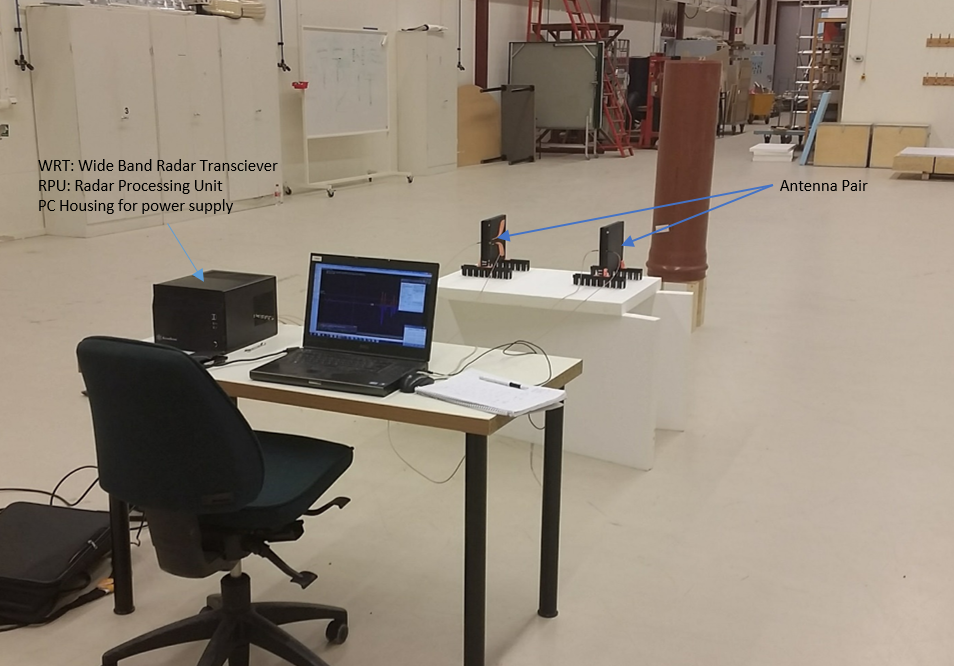
\includegraphics[width=\linewidth]{Figures/RadarMeasurement.png}
    \caption{UWB radar measurement system: WRT and RPU in a PC housing}
    \label{fig:RadarPic}
\end{figure}

\subsection{Software Platform}
A windows application for data acquisition and processing is designed and implemented at Addiva AB. Although the radar system is delivered with a windows application for data acquisition and processing, every new algorithm should have been coded in C to be able to test on live radar data. The idea behind designing this application is to create a platform to be able to directly use thousand of MATLAB algorithms and libraries for signal processing. The radar system is connected to the PC via a USB port. The software platform acquire the raw data produced by the radar system and a MATLAB core is used to process the data. The platform is built in a way that the algorithm parameters and their sequence is editable in the user interface. The raw radar data plus the processed data are shown together in the same window. Using MATLAB as a core gave us access to the advanced and computationally enhanced signal processing algorithms to be applied directly on the live, raw data and it decreases the time from idea to result. An overview of the system is shown in figure \ref{fig:system}.
\begin{figure}
    \centering
    \hspace*{-2cm} 
    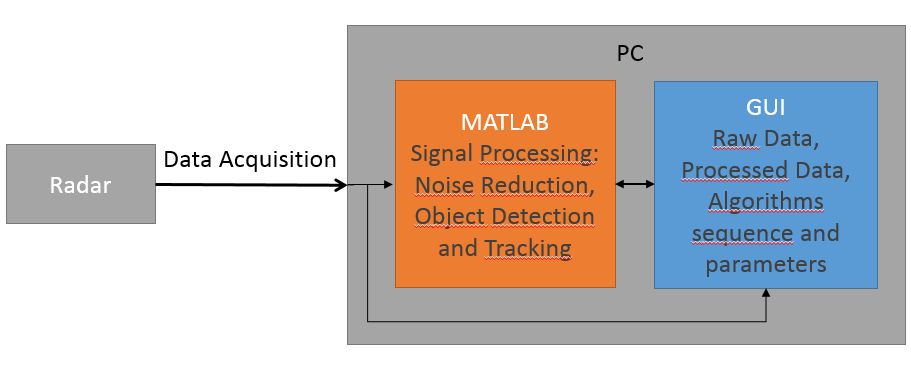
\includegraphics[width=100mm]{Figures/System.PNG}
    \caption{Data Acquisition and processing System}
    \label{fig:system}
\end{figure}

To ease the prototyping and experimentation process the application software has a specific architecture. Data acquisition and GUI software are developed in C\# and the signal processing algorithms are developed in Matlab\textsuperscript{TM} then an API connects Matlab\textsuperscript{TM} code to the GUI so after building DLLs it is possible to run the developed algorithms with real system. Matlab\textsuperscript{TM} is a prototyping platform with thousand of ready libraries and function which makes development and testing of algorithms faster. A screenshot of the application is shown in Figure 
\begin{sidewaysfigure}
    \centering
    %\hspace*{-2cm} 
    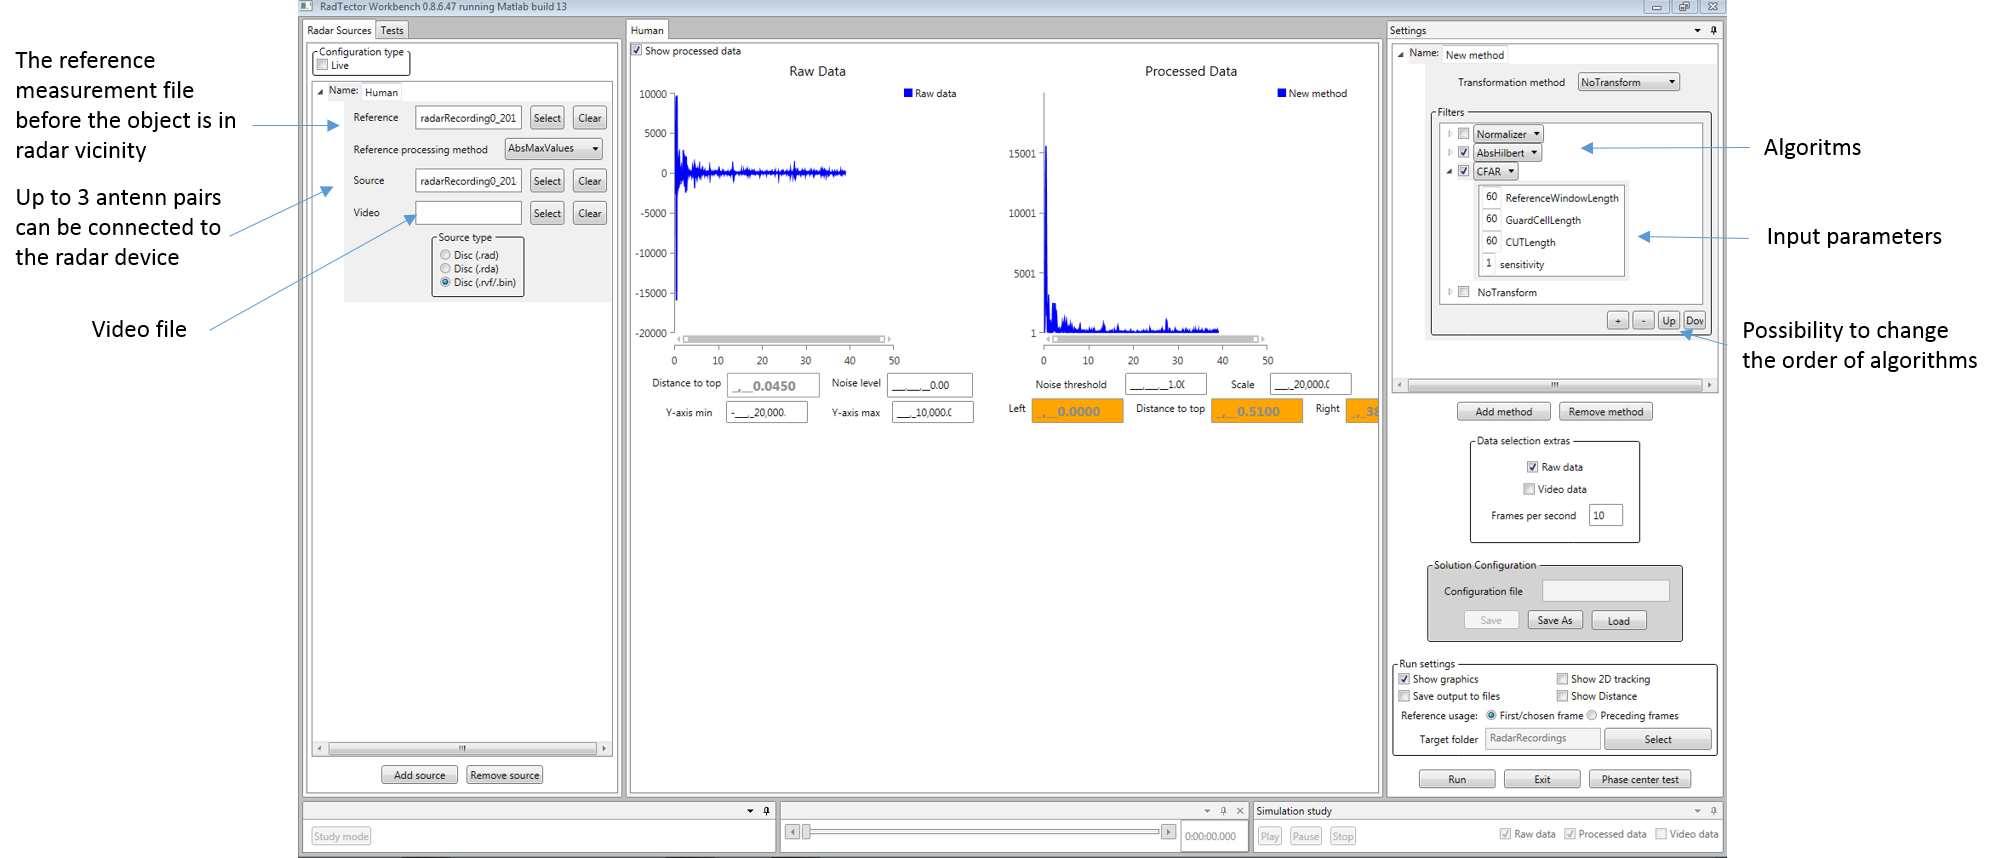
\includegraphics[width=20 cm,keepaspectratio]{Figures/RadTector.PNG}
    \caption{Data acquisition and processing application}
    \label{fig:RadTector}
\end{sidewaysfigure}
\subsection{Data Representation}
The radar system is able to record hundreds of scans per second. Theses results are presented in two ways: either just a returned wave of the radar at a certain time is shown such as Figure \ref{fig:RadarReturnSignal} or the radar returns are stack along the time axis. This result in a two-dimensional graph which is called radargram. The structure of radargram is shown in Figure \ref{fig:Radargram} and an example of real measurements are shown in Figure \ref{fig:BreathingSimulationResults}.

\begin{figure}
    \centering
    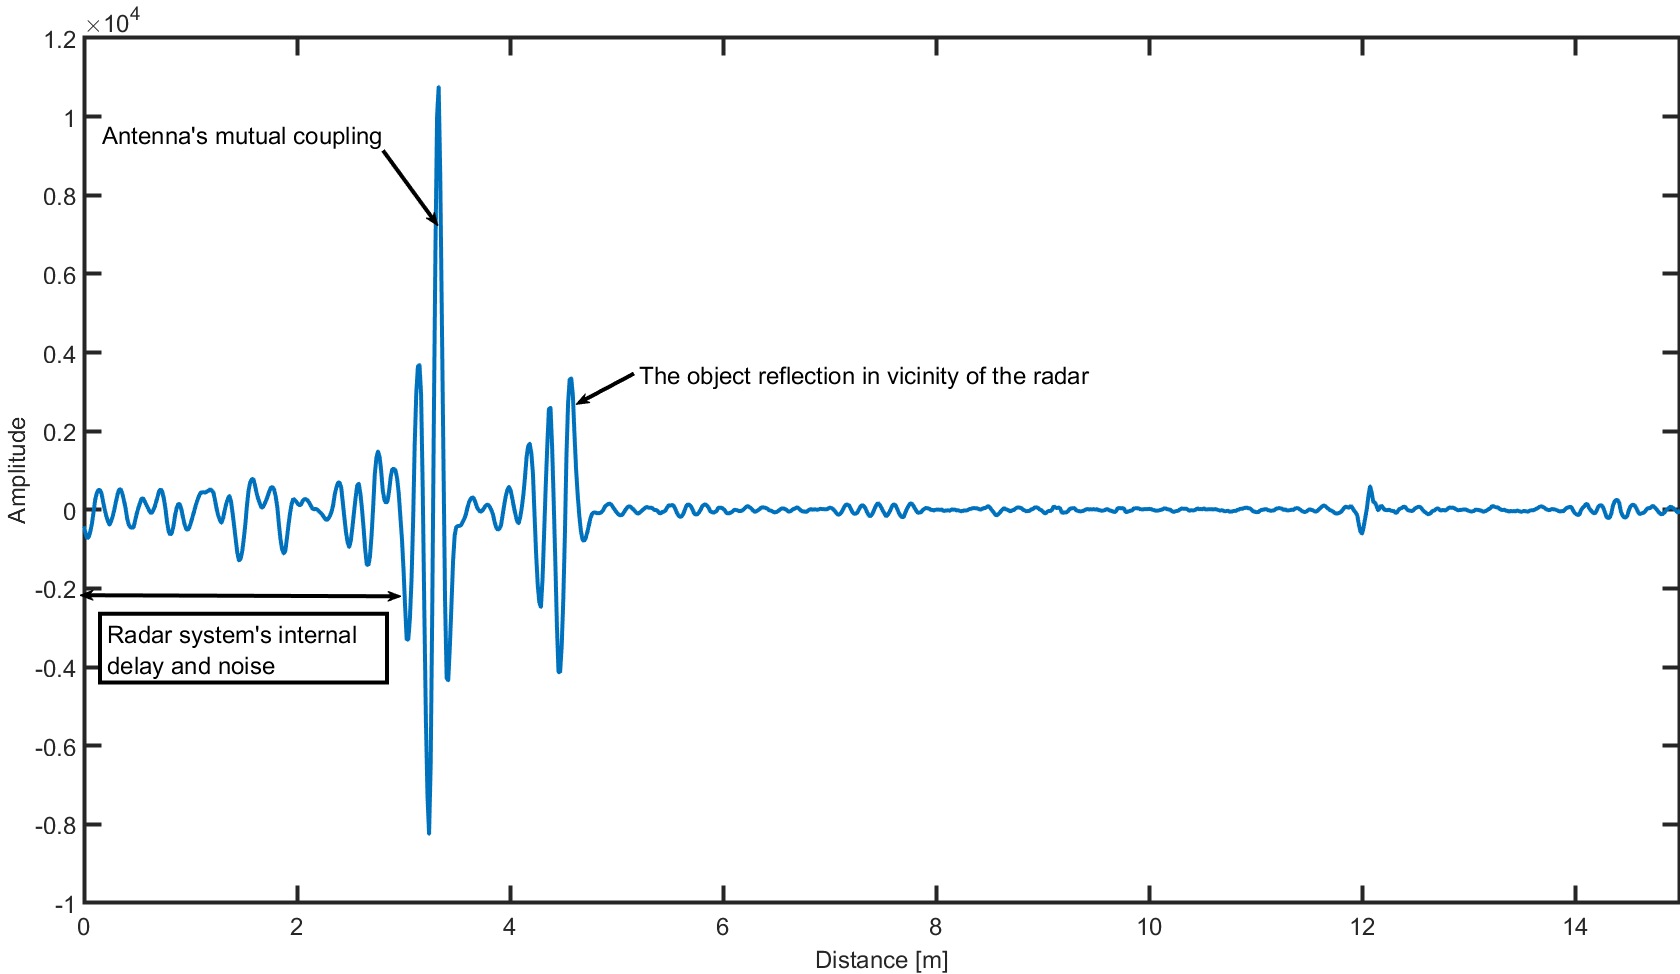
\includegraphics[width=\linewidth]{Figures/RadarReturnSignal.png}
    \caption{Radar's return signal}
    \label{fig:RadarReturnSignal}
\end{figure}
\begin{figure}
    \centering
    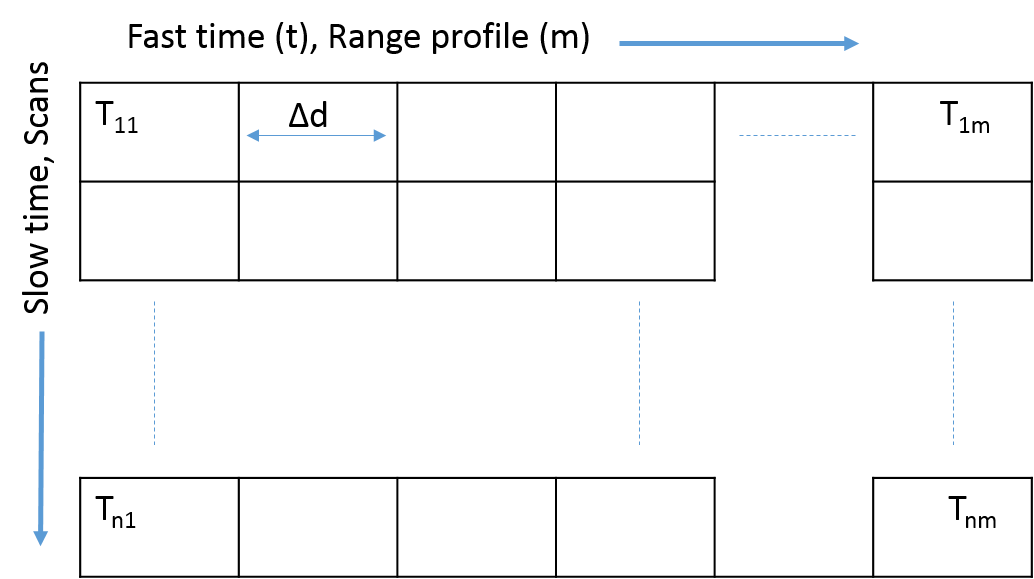
\includegraphics[width=\linewidth]{Figures/RadarReturnSignal2D.png}
    \caption{Radargram structure}
    \label{fig:Radargram}
\end{figure}
%%%%%%%%%%%%%%%%%%%%%%%%%%%%%%%%%%%%%%%%%%%%%%%%%%%%%%%%%%%%%%%%%%
\section{System Evaluation and Measurements}
For this thesis many measurements are performed to understand the system constraints, characteristics and abilities. In this section some of these measurements are presented.
\subsection{Vivaldi Antenna Radiation Pattern: Simulations and Measurement}
In this section an overview of simulation and measurement of the Vivaldi antenna used in this project is presented. The antenna pattern is an important factor in radar measurements to understand the interaction with the equipment or human under test.

The antenna was simulated in CST studio suit\textsuperscript{TM}. The result of the simulation is shown in Figure \ref{fig:Simulation_1G} and \ref{fig:Simulation} 
\begin{figure}[!]
    \centering
    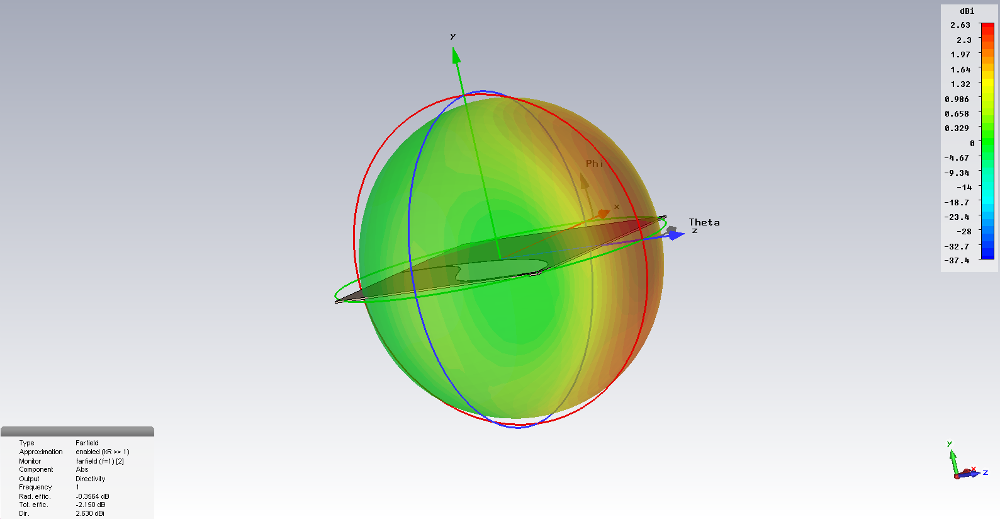
\includegraphics[width=100mm]{Vivaldi/farfield1GScale.PNG}
    \caption{Simulation of Vivaldi antenna in CST studio\textsuperscript{TM}}
    \label{fig:Simulation_1G}
\end{figure}

\begin{figure}
    \centering
    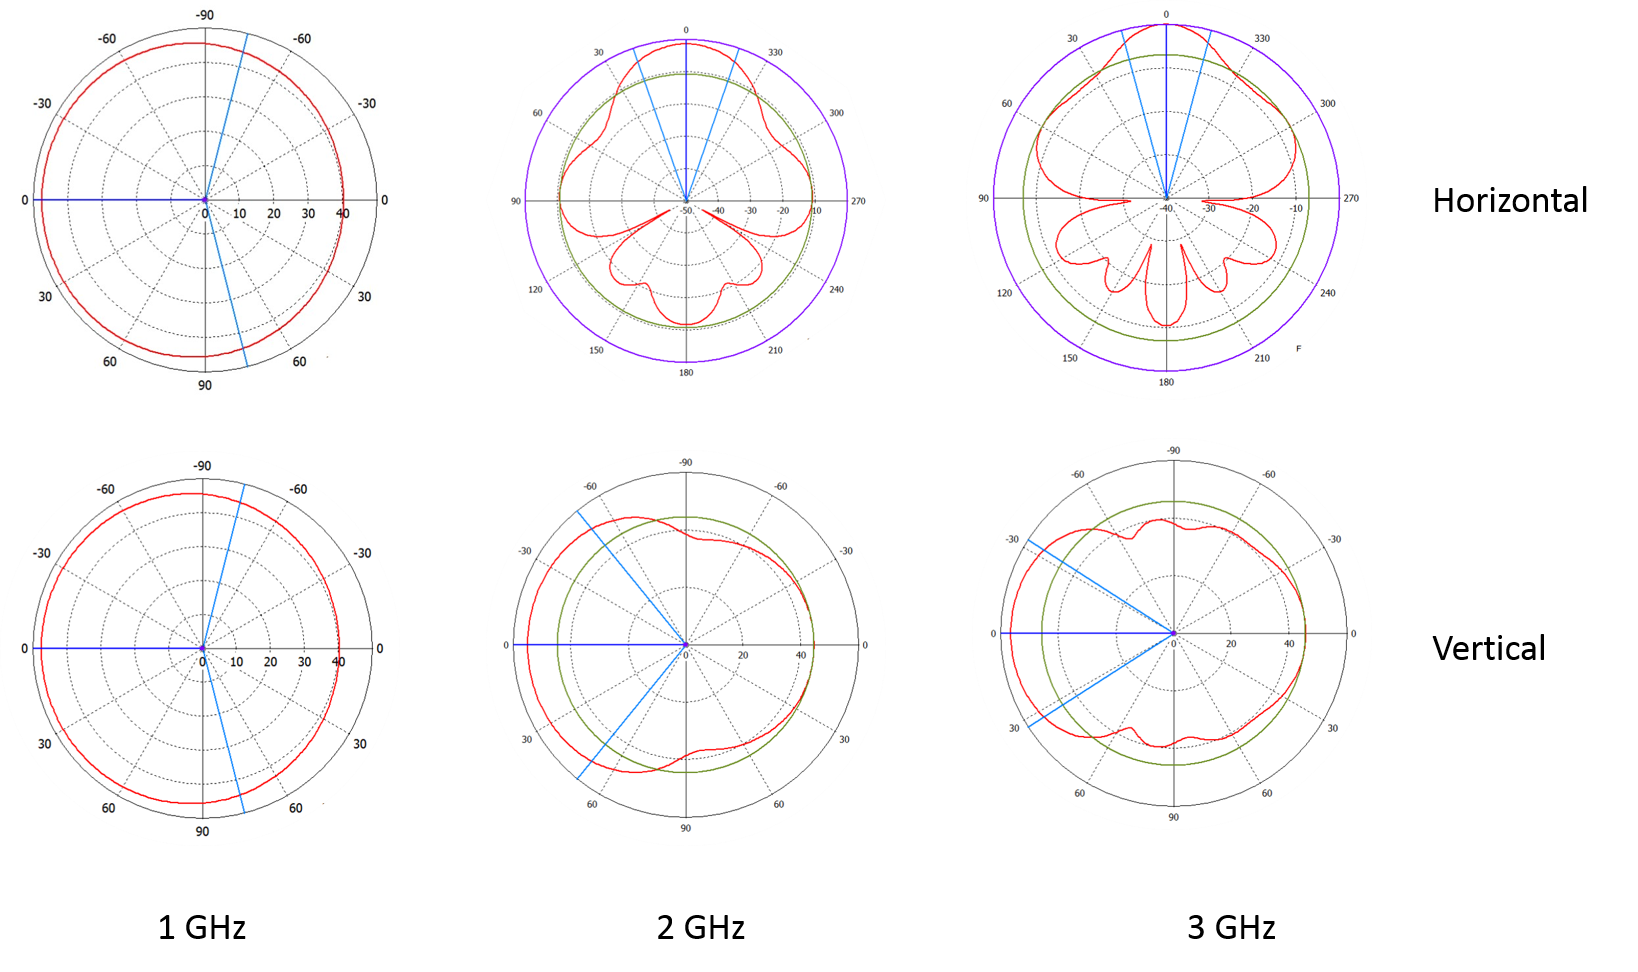
\includegraphics[width=100mm]{Vivaldi/SimulatedAntennas.PNG}
    \caption{Vertical and horizontal polarization of Vivaldi antennas in simulation}
    \label{fig:Simulation}
\end{figure}

The Vivaldi antenna's radiation pattern is measured in an anechoic chamber in DELTA Development Technology by great-circle method \cite{FoegelleAntennaPattern}. In this method the Measurement Antenna (MA) which is the Horn antenna is fixed and the Antenna Under Test (AUT) which is the Vivaldi antenna is placed on a rotational positioner and rotated about the azimuth through 360\textdegree~to generate a two-dimensional polar pattern. The rotational positioner is circulating in 5\textdegree~steps.  The measurement is repeated when the Vivaldi antenna is manually rotated 90\textdegree   to measure the horizontal polarization.

The antennas positioned on 3 meters height to reduce the reflection from the floor. A balun with 3dB damping following by a pair of semi rigid coaxial cables connects the Vivaldi antenna to a synthesized sweeper that generates CW waves from 1-3 GHz with the step of 1 GHz. A horn antenna with an inbuilt amplifier is connected to an electromagnetic interference (EMI) test receiver. 
%The resolution bandwidth(RBW) is 1 MHz and video bandwith(VBW) is 3 MHz span 50 MHz SNR ca 40 dB cneter ferquency 2 Ghz Amplitude enher dBmicrovolt: decible of the RMS micro volt dB\micro V= 20Log(\micro V),,,,Genetaror 2 Ghz and -20 dBm
\begin{figure}[t] 
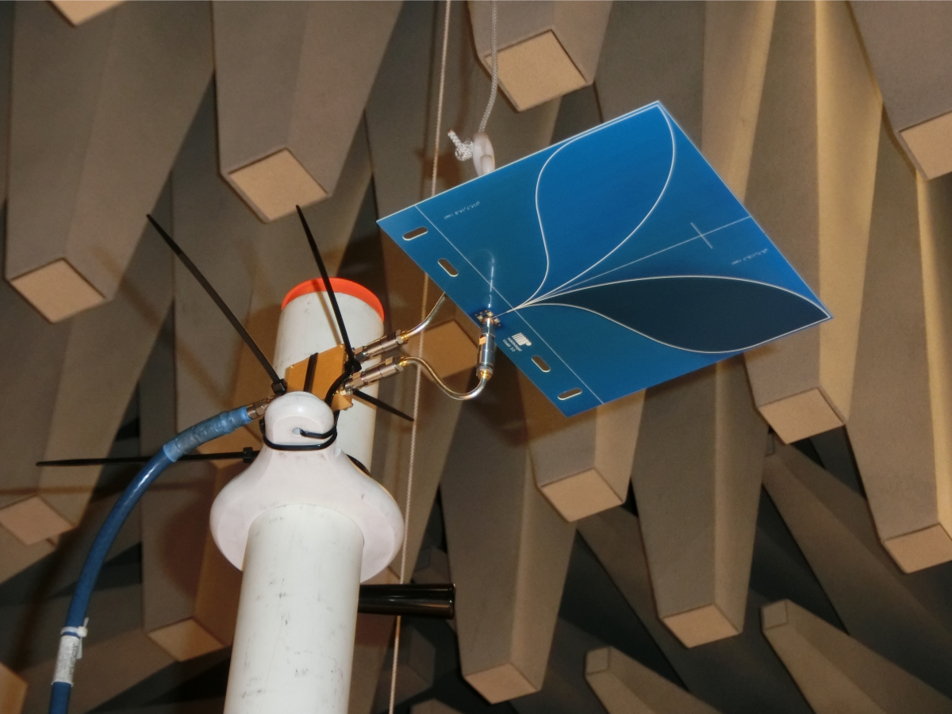
\includegraphics[width=\linewidth]{Figures/vivaldiHorizontal.png}
\caption{Vivaldi antenna connected } 
\label{fig:MeasuredAntenna}
\end{figure}


\begin{figure}[t] 
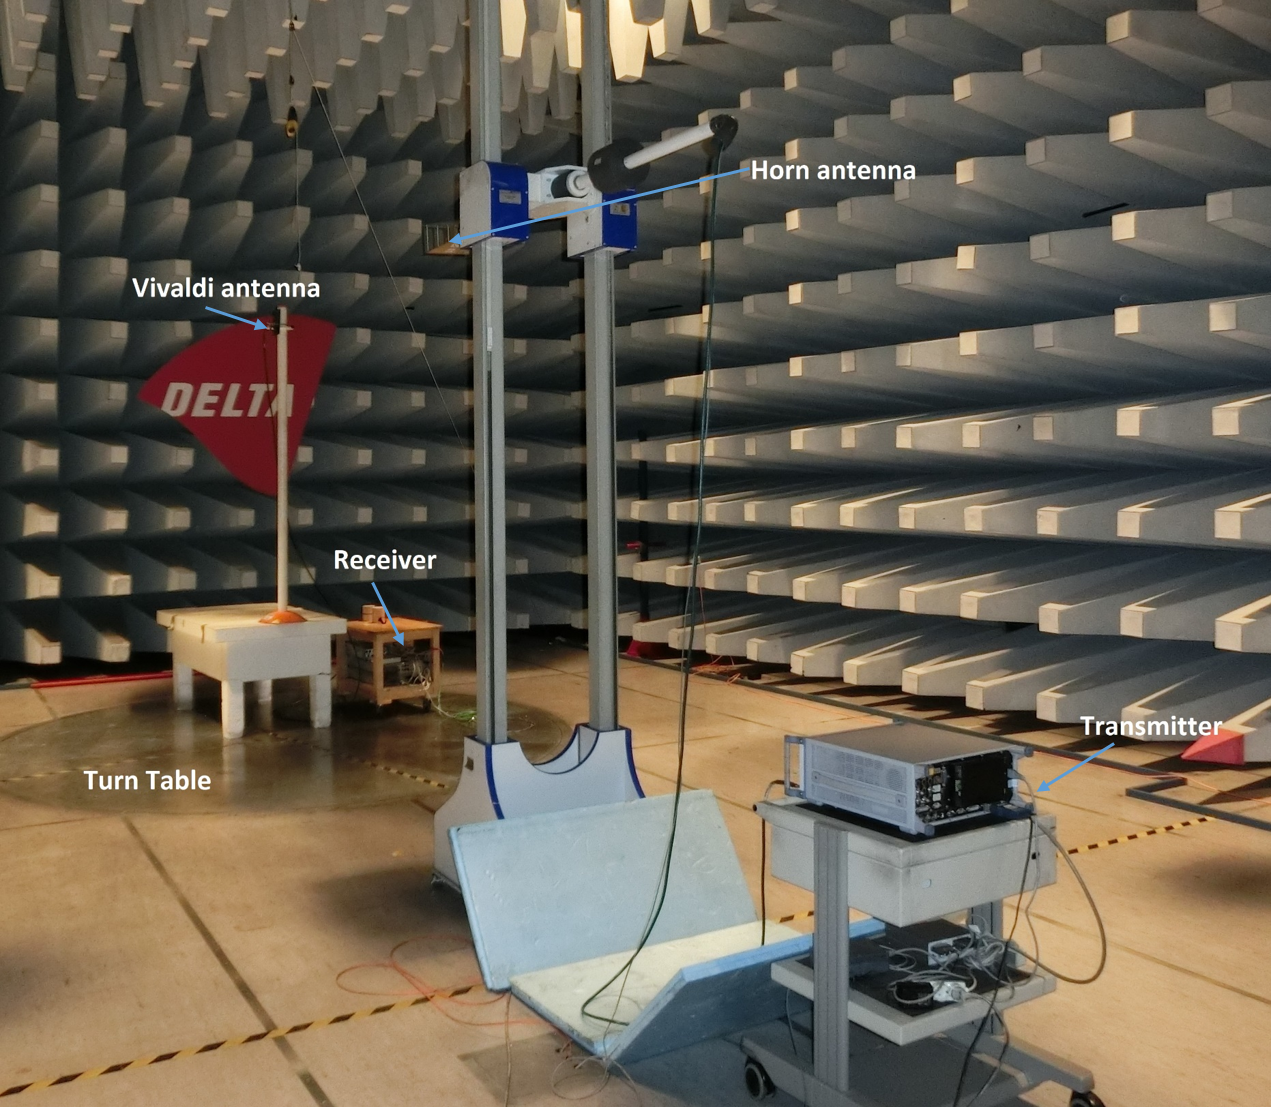
\includegraphics[width=\linewidth]{Figures/AntennaMesearment.png}
\caption{Vivaldi antenna radiation pattern measurement} 
\label{fig:MeasuredAntenna}
\end{figure}
The results are for both horizontal and vertical polarization. The results is shown in figure \ref{fig:MeasuredAntenna}
\begin{figure} 
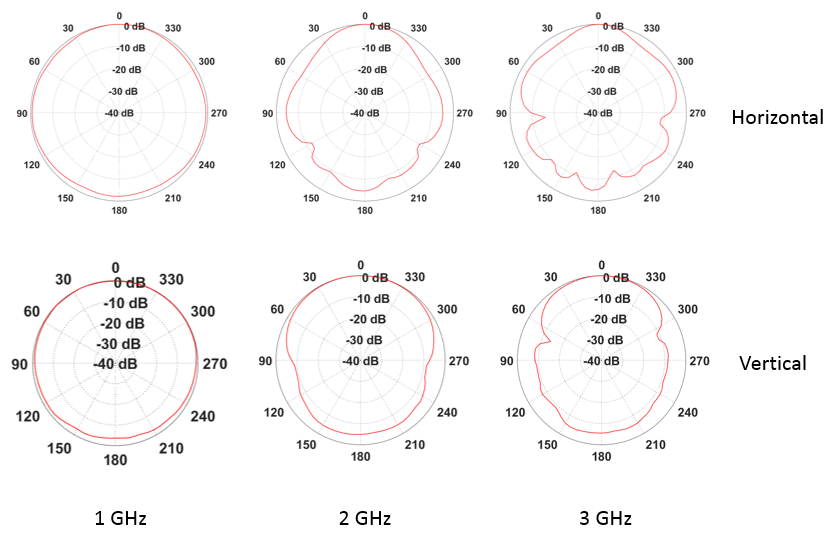
\includegraphics[width=\linewidth]{Vivaldi/MeasuredAntennas.PNG}
\caption{Measured antenna } 
\label{fig:MeasuredAntenna}
\end{figure}

\subsection{Antenna phase center}
 In order to do fine measurement and tuning of the system an xy board is developed. The xy board is a aluminium structure with two dimensional movement possibility. The step-motors in every dimension are very precise and have mm precision. The motors are driven by a 3D printer program and raspberry pie (Arduino).
 \todo{make you own picture}
The phase center of an antenna is defined as the apparent source of radiation. By knowing the phase center of the antenna the precise measurements does not need calibration.
The experimental setup had been done base on the approach presented in \cite{liu2013phase}. The two antennas paced in the bore sight direction of each other and the receiver antenna moved in 5 mm steps in x direction  on xy board. The transmitted signal is recorded at every step.
\begin{figure}
    \centering
    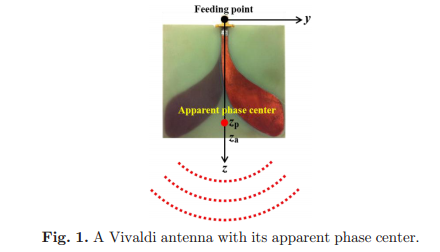
\includegraphics{Vivaldi/phase center.jpg}
    \caption{phase center\todo{change this picture to our own antenna}}
    \label{fig:my_label}
\end{figure}
We decided to do a modification here to the original and based the whole equation just on distances and not the time ($\tau_p$ is the time that the wave travels from feeding point to the edge of the antenna.)
\todo{add the results if you find the error otherwise remove this subsection}
\begin{figure}
    \centering
    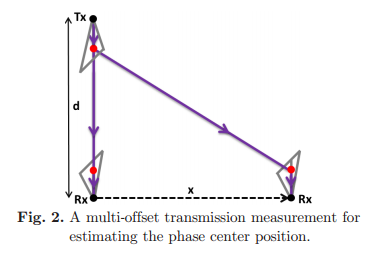
\includegraphics{Vivaldi/phasecenter2.png}
    \caption{}
    \label{fig:my_label2}
\end{figure}

\subsection{Reflector Design}
 The reflector can be used for different purposes, but two main application areas are : Usage as an artificial target with applications in radar calibration and usage to extent the radar range when carried by the target.
This section describes how the non amplified radar reflector circuit is connected. This circuit powers the receiver antenna and connects the signals coming from the receiver antenna to the transmitter antenna.
The circuit is powered with +5V, -5V and GND. The circuit takes its inputs via one RJ45 connector that is to be connected to the receiver antenna. The circuit gives its outputs via one RJ45 connector that is to be connected to the transmitter antenna.
\todo{schematics can be added}
\subsection{Breathing Simulation}
The movement of the chest is simulated by a xy board. The antenna pair, sender and receiver are placed on a stand and an aluminium plate 20*20 cm is moved periodically for 2 cm 90 degrees to bore sight of the antennas. The set-up is shown in Figure \ref{fig:BreathingSimulation}.
\todo{add axis properties}
\begin{figure}
    \centering
    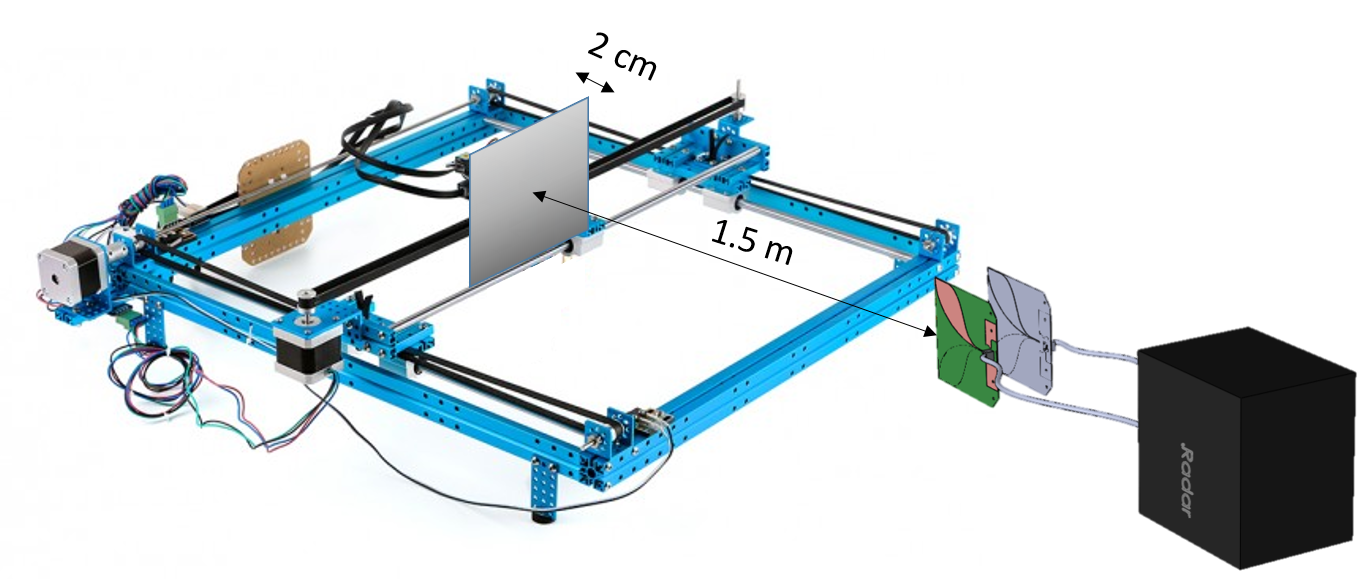
\includegraphics[width=\linewidth]{Figures/BreathingSimulation.PNG}
    \caption{Breathing Simulation Set-up}
    \label{fig:BreathingSimulation}
\end{figure}
The results are shown in Figure \ref{fig:BreathingSimulationResults}
\begin{figure}
 \centering
  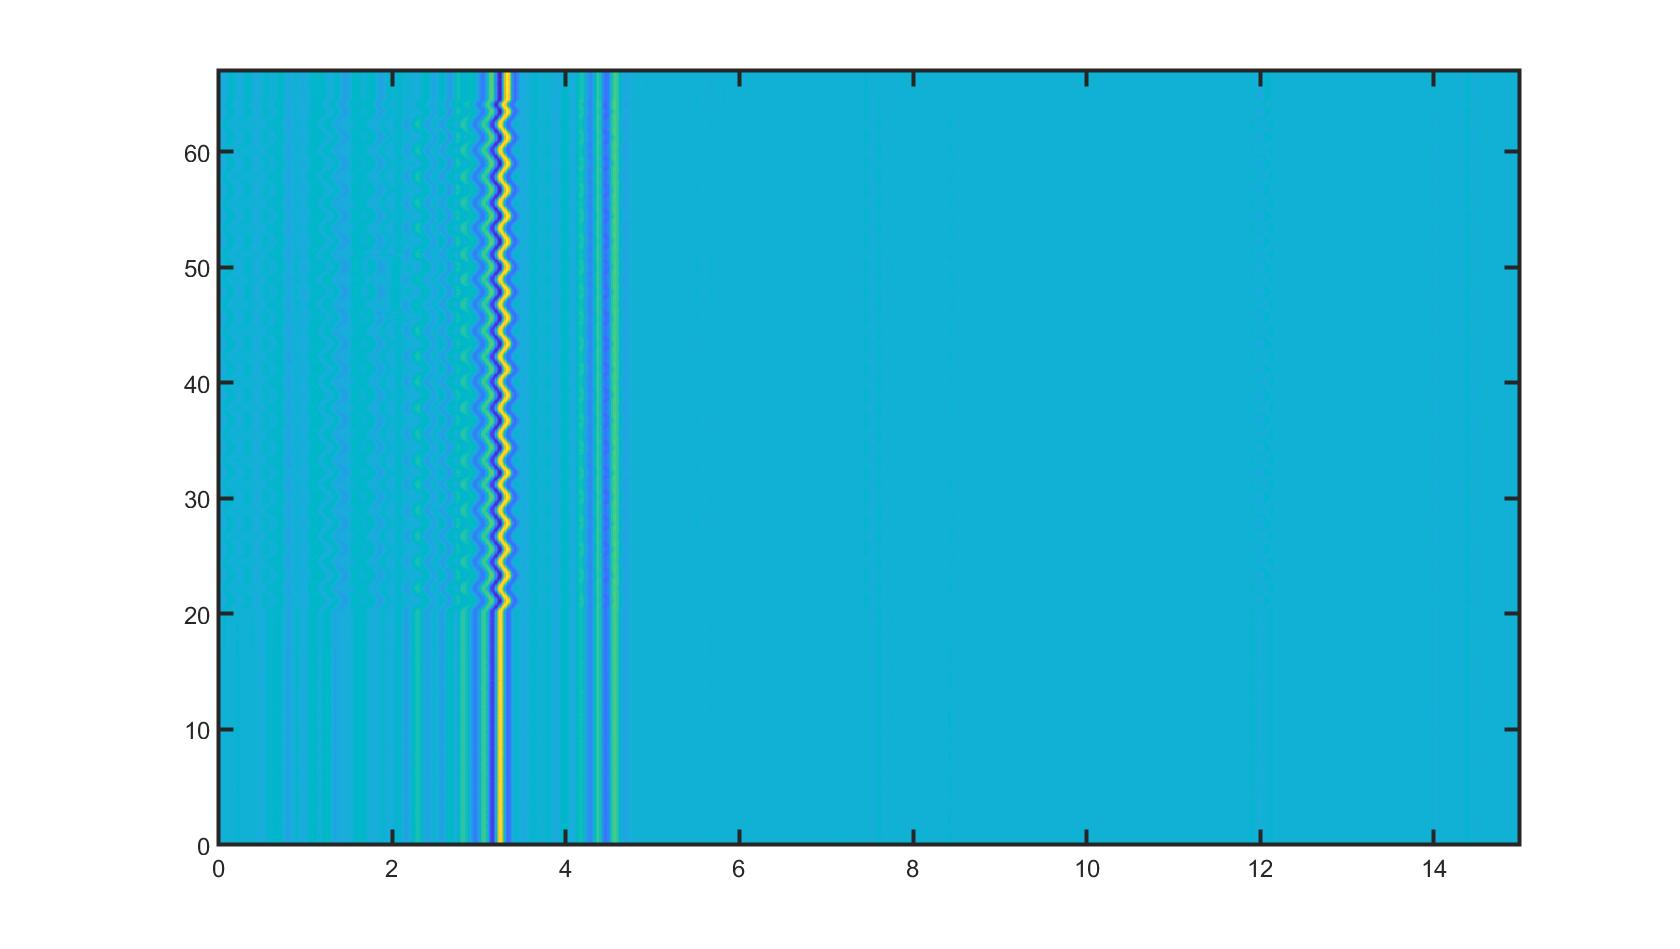
\includegraphics[width=\linewidth]{Figures/SimulationResult.jpg}
\caption{Breathing Simulation Results}
\label{fig:BreathingSimulationResults}
\end{figure}
The measurement is repeated with a real human sitting in-front of the radar and breathing normally. To detect human breathing needs further investigations.

\section{Signal Processing Algorithms}
A series of signal processing algorithms was developed mainly to be able track the target movements. These stages are summarized below.  The delay introduced by the electronic circuits is removed from the raw radar scan before the processing. The amount of delay is easy to recognize by the large reflection caused by the mutual coupling.
\subsection{Pre-processing}
The main objective for pre-processing is to remove noise from  the raw signal.  
\begin{itemize}
    \item {Hilbert Transform}
    Hilbert transform is used for enveloping the signal and reduce the noise. Hilbert transform is showing the complex envelope representation of the signal. The result of the transform is shown in Figure \ref{fig:Hilbert}. Hilbert transform makes it easier to find the peaks in the signal.
\begin{figure}
    \centering
    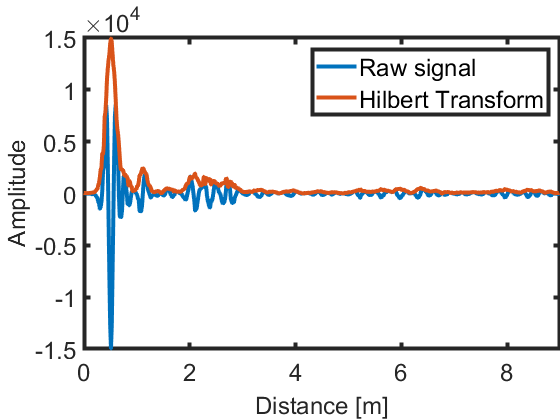
\includegraphics[width=\linewidth]{Figures/Hilbert.png}
    \caption{Absolute value of the Hilbert transform of the signal}
    \label{fig:Hilbert}
\end{figure}
    \item Automatic Noise reduction: This filter sets a limit based on the standard deviation of the data. Any data point with an absolute value less than this value gets zeroed. The function gets the sensitivity as an input argument.\\
    \hspace*{7mm} result(abs(result) $<$ standard deviation * sensitivity
\end{itemize}
\subsection{Background Removal Methods}
Background is everything in the vicinity of radar but the object of  interest. To remove background from the radar data two approaches are tested: In case of an static object a reference measurement is performed before the object of interest is placed in the radar vicinity. Although the Object reflections is not equal to Reflection minus reference due to ?\todo{find the terms for this} measurement.
For dynamic objects it is possible to used the first (seconds) of radar measurement as the reference measurements. Following these empirical trials are presented  
\begin{itemize}
    \item{Averaging}: This method makes the reference frame simply by averaging every point in reference measurement and removing it from every frame in measurement data.
   % \item {Adaptive Reference} 
   % result[i] = $\alpha$  * result[i-1] + (1 - $\alpha$ ) .* data
    \item Adaptive Background Subtraction: 
    This method is implemented based on the method presented in \cite{Zetik}. This method has the advantage of removing the background from measurements where human detection is based on breathing or smaller movements when other background removal methods remove these small movement as they are static backgrounds. In this method $\alpha$ is not a scalar value but a vector of weighing coefficients $\alpha_k$. This vector is time variant where $k$ is a certain time instance. Vector $q_k$ is adapting the $\alpha_k$ coefficients. The following lines shows how $\alpha$ is changed in an adaptive way.
 
        \hspace*{5mm}if $q_{ik} < Threshold_1$\\
          \hspace*{15mm} if $q_{ik}/z_{ik} < Threshold_2$\\
               \hspace*{25mm}$ \alpha_{ik} = 1;$\\
            \hspace*{15mm}else\\
                \hspace*{25mm}$\alpha_{ik} = \alpha;$\\
       \hspace*{5mm} else\\
              \hspace*{15mm}$\alpha_{ik} = 1;$\\
  

    \item{Removal of absolute maximum}:  
    To make the reference frame the the absolute maximum of every point in reference measurement is founded. This method can help removing those high peaks showing up in frames due to noise. At the same time it might remove the important data. This method is good when an activity or movement shall be detected.
    \todo{refer to \ref{fig:Radargram}}
    \item Median Removal: In this method the median of reference measurement is removed from the measurement frames
    \item Fast and slow averaging: Applying one slow moving averaging filter and one fast moving averaging filter. 
       $ y[i] := \alpha * x[i] + (1-\alpha) * y[i-1]$
%  The result is the difference between the two filters
\end{itemize}
\subsection{Target detection}
Detection algorithms will determine if the target is absent or present in radar signal.
\begin{itemize}
    \item CFAR: Cell averaging CFAR (Constant False Alarm Ratio) Detector that belongs to the category of sub-optimum detectors. CFAR detectors are provide adaptive estimation of an optimum threshold based on Neyman-Pearson criterion and assuming, that the probability distribution function of the clutter is known \cite{CFAR2010}. CFAR is an adaptive procedure that detect the targets by compare the neighboring cells to the neighboring cells. The advantage of this method is that it in an adaptive way keeps the probability of false alarm at a constant value. The decision about if a cell is a target or not is based on a statistical decision theory. An overview depiction of CFAR is presented in Figure \ref{fig:CFAR}.\todo{complete the figure}
        \begin{figure}[t]
            \centering
            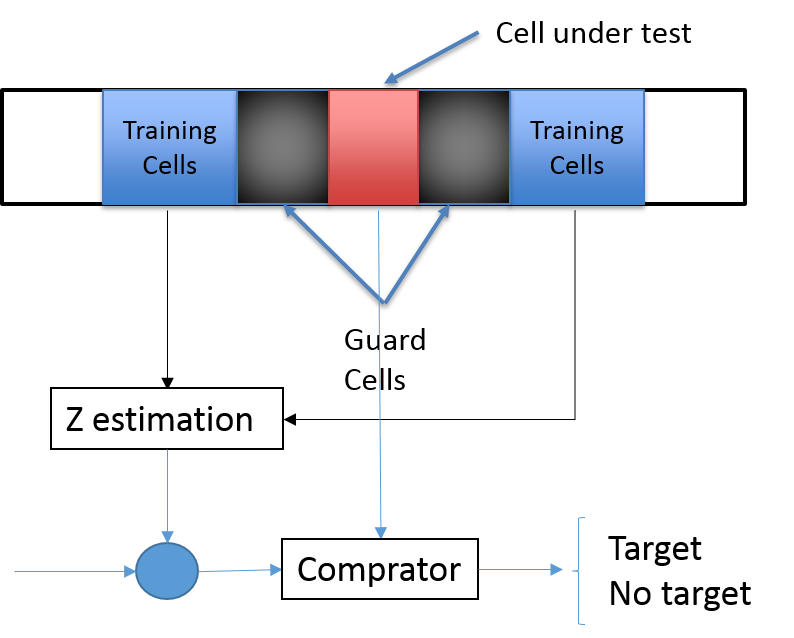
\includegraphics[width=\linewidth]{Figures/CFAR.png}
            \caption{CFAR processing}
            \label{fig:CFAR}
        \end{figure}
    \item Peak detector:  This method simply detect the peaks in the data based on a certain limit and present them as potential targets.
\end{itemize}
\subsection{Target Tracking}
The target tracker is designed based on detection of peaks that are greater than a certain limit or having the integral under the peaks greater than a limit. A flow chart of this algorithm is shown in \ref{fig:FlowChart}.
\begin{figure}
    \centering
    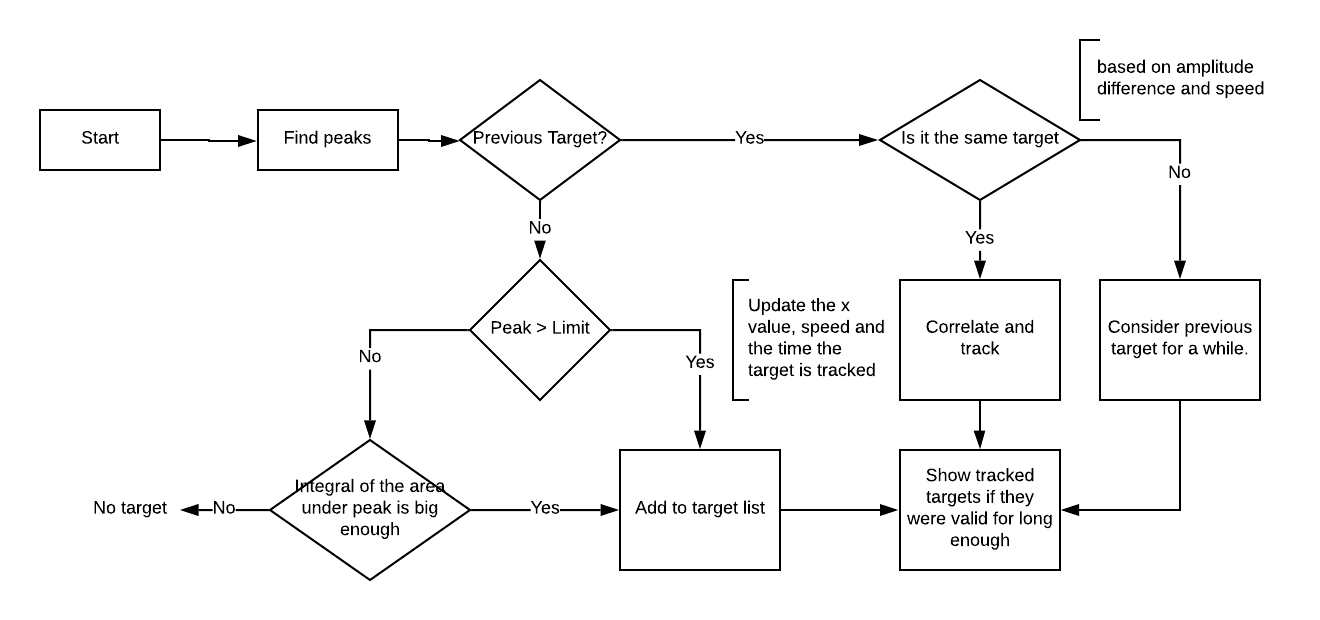
\includegraphics[width=10 cm]{Figures/BlankDiagram.PNG}
    \caption{Flow chart of the target tracker algorithm}
    \label{fig:FlowChart}
\end{figure}
\subsection{Other Algorithms}
Some algorithms are developed for other use that target detection and tracking. Two of these algorithms are presented below.
\subsubsection{Distance Modulation}
Distance Modulation  modulates the data to get its amplitudes to be independent of distance i.e. echos from far shall be able to "compete" with echos from near. This is mostly due to a better representation of the targets at further distances. It has been observed that the modulation is not linear by measurements of a metal plate at different distances. In the next step the points are drawn from measurements and a fit function from MATLAB could estimate the function which is the following polynomial:
$1461 * xdata .^2 - 9119 * xdata + 15687$ 
\subsubsection{Increasing precision by re-sampling}
Due to the stability of the signal in x-axis by re-sampling the signal it is possible to reach a better accuracy. Theoretically the radar range resolution is 7.5 cm based on the center frequency. By re-sampling the signal 20 times it was possible to reach around 3 mm precision in range resolution.  
%\section{Cable Measurements}
%\section{Receiver Sensitivity }